
\documentclass[a4paper]{article}
%\pgfplotsset{compat=1.12}
%\usepackage{conference}
\usepackage{latexsym}
\usepackage[perpage,symbol*]{footmisc}
\usepackage[utf8x]{inputenc}
\usepackage[english]{babel}
\usepackage{amssymb,amsfonts,amsmath}
\usepackage{xcolor}
\usepackage{tikz}
\usepackage{tikz-3dplot}
\usepackage{pgfplots}
\usepackage{pgfplotstable}
\usepackage{cite}
\usepackage{hyperref}
\usepackage[varg]{txfonts}
\usepackage[T1]{fontenc}                   % Font encoding
\usepackage{geometry}
 \geometry{
 a4paper,
 total={170mm,257mm},
 left=20mm,
 top=20mm,
 }
%%%%%%
%%%%%%
\usetikzlibrary{patterns,arrows.meta,shapes,calc,angles,positioning,intersections,through,quotes,decorations.markings}
%\tdplotsetmaincoords{70}{110}
\usepackage{tkz-euclide}
\usetkzobj{all}
%%%%%%%
\def\doubleunderline#1{\underline{\underline{#1}}}
%%%%%%%
%%%%%%%

%% Begin of Watermark feature
%\usepackage[printwatermark]{xwatermark}
%\usepackage{xcolor}
%\newwatermark[allpages,color=red!50,angle=60,scale=6,xpos=0,ypos=0]{DRAFT}
%\newwatermark[allpages,color=red!20,angle=60,scale=2,xpos=0,ypos=0]{For Peer Review}
%% End of Watermark feature

\begin{document}

\title{Topological Axis in Macro and Micro \emph{physics}}


\begin{table}

\centering
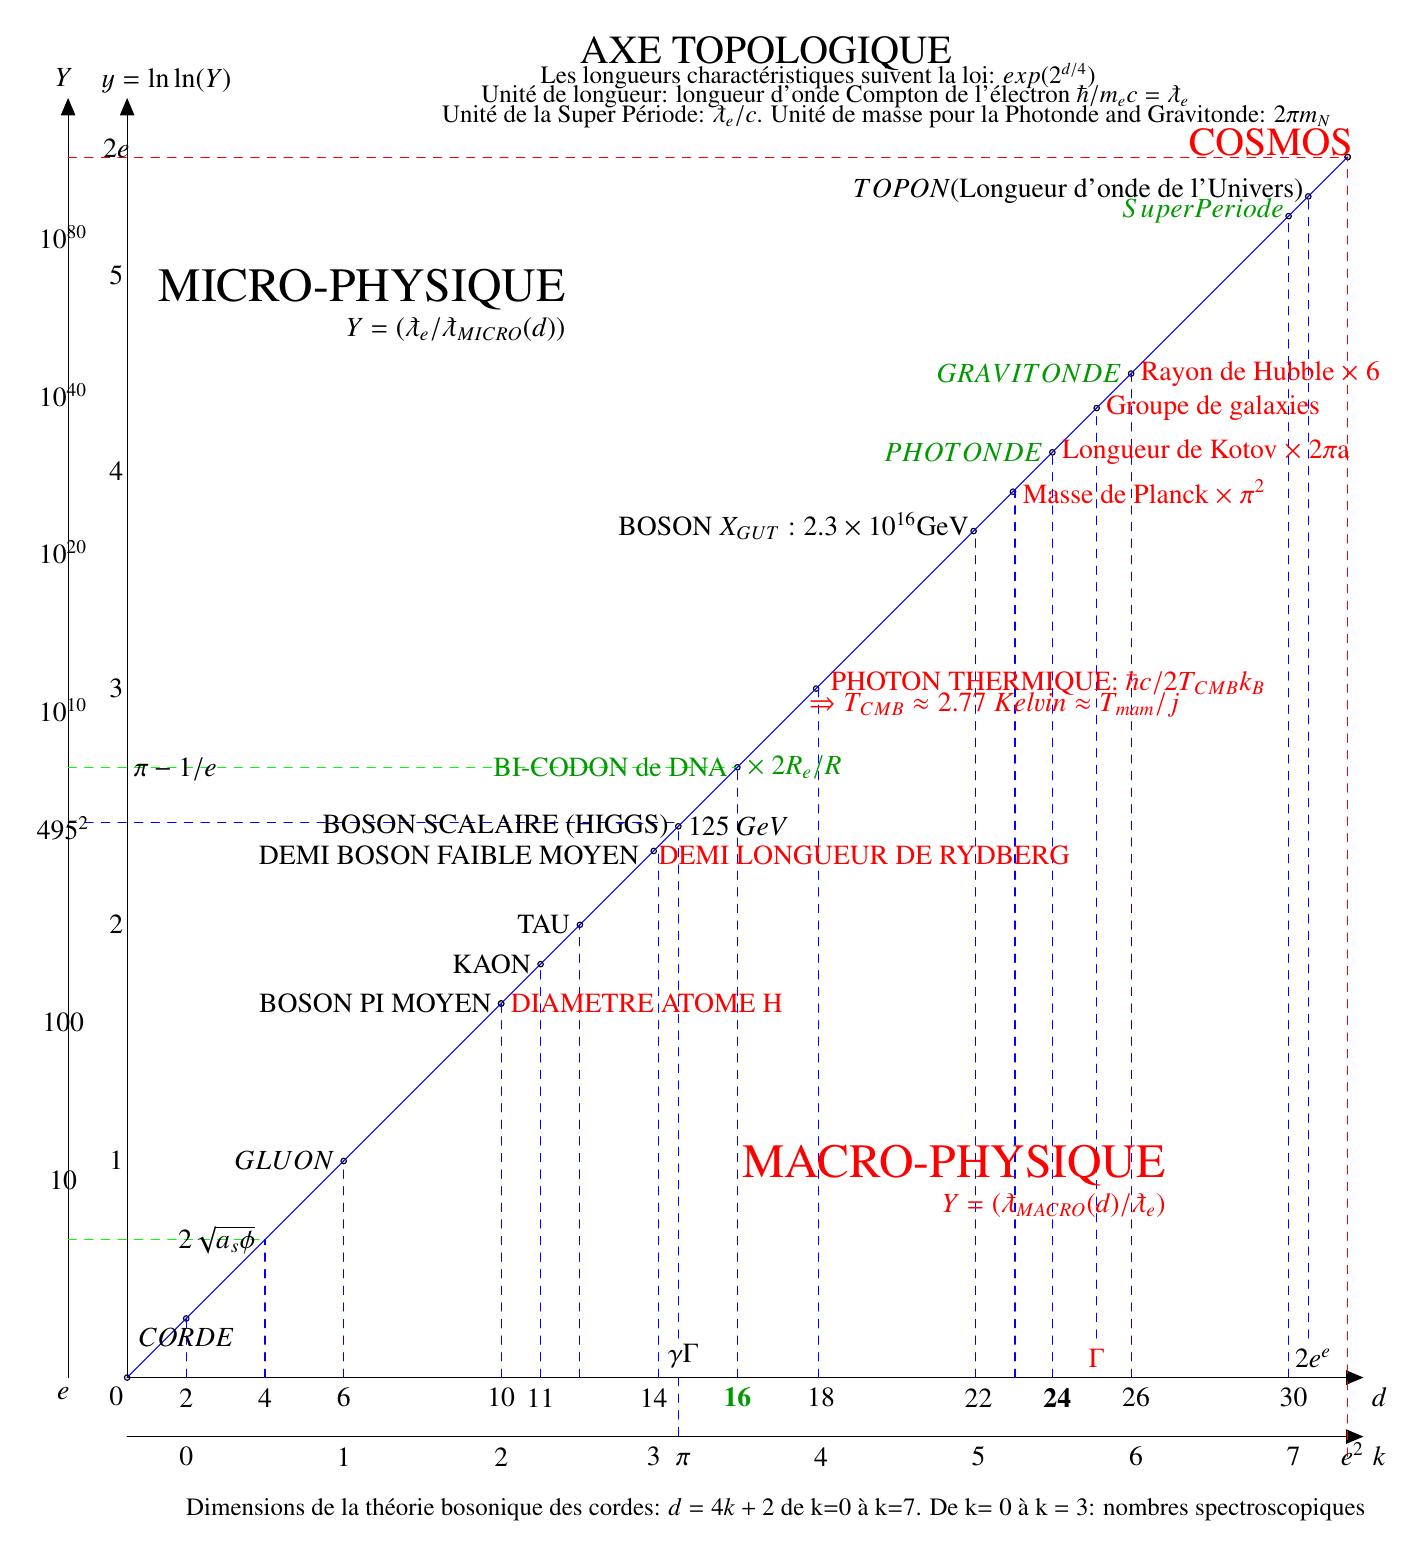
\begin{tikzpicture}[line cap=round,line join=round,>=triangle 
45,x=0.25cm,y=0.25cm]

\tkzDefPoint(-31.0,-31.0){A} %\tkzDefPoint(5.,3.43){B} \tkzDefPoint(5.,0.){C} \tkzDefPoint(31.0,31.0){Y}
\tkzDefPoint(-28.0,-28.0){B}
\tkzDefPoint(-20.0,-20.0){C}
\tkzDefPoint(-12.0,-12.0){D}
\tkzDefPoint(-12.0,-12.0){E}
\tkzDefPoint(-8.0,-8.0){R}
\tkzDefPoint(28.0,28.0){F}
\tkzDefPoint(-4.25,-4.25){G}
\tkzDefPoint(4.0,4.0){H}
\tkzDefPoint(12.0,12.0){I}
\tkzDefPoint(14.0,14.0){S}
\tkzDefPoint(-3.0,-3.0){J}
\tkzDefPoint(16.0,16.0){K}
\tkzDefPoint(18.25,18.25){L}
\tkzDefPoint(20.0,20.0){M}
\tkzDefPoint(29.0,29.0){N}
\tkzDefPoint(-10.0,-10.0){P}
\tkzDefPoint[color=red](31.0,31.0){Q}
\tkzDefPoint(31.0,31.0){Y}
\tkzDrawPoints(A,B,C,D,F,E,G,H,I,J,K,L,M,N,P,Q,R,S,Y)
%\tkzMarkRightAngle(A,D,C)
%\tkzLabelPoints[text=red,right](G,H)
%\tkzMarkAngle[fill=blue!40,size=1.4cm,opacity=.5](C,A,B)
%\tkzLabelAngle[pos=1.6](C,A,B){$\theta$}
\tkzDefMidPoint(A,Y) \tkzGetPoint{BI-CODON}
\coordinate (center) at (BI-CODON);
%\tkzLabelPoints[below,color=green](BICODON)
\tkzDrawPoints(BI-CODON)
\draw [->] (-31.0,-31.0) node[left]{} -- (-31.,34.) node[right]{}; % scale Y
%\draw [->] (31.0,-31.0) node[left]{} -- (31.,31.) node[right]{}; % 
\draw [->] (-31.0,-31.0) node[left]{} -- (31.8,-31.0) node[right]{}; % scale d
\draw [->] (-31.0,-34.) node[left]{} -- (31.8,-34.) node[right]{};   % scale k
\draw [->] (-34.0,-31.) node[left]{} -- (-34.,34.) node[right]{};   % scale Y'
%%% Blue Dashed Horizontal lines
\draw [-,color=green,dashed] (-34.0,-24.) node[left]{} -- (-24.,-24.) node[right]{};   % \sqrt{a_s} horizontal line
\draw [-,color=blue,dashed] (-34.0,-2.8) node[left]{} -- (-2.8,-2.8) node[right]{};   % Scalar Boson horizontal line
\draw [-,color=green,dashed] (-34.0,0.) node[left]{} -- (0.,0.) node[right]{};   % bicodon horizontal line
\draw [-,color=red,dashed] (-34.0,31.) node[left]{} -- (31.,31.) node[right]{};   % Cosmos horizontal line
%%% Blue Dashed Vertical lines
\draw [-,color=blue,dashed] (-28.0,-31.) node[left]{} -- (-28.,-28.) node[right]{};   % String vertical line
\draw [-,color=blue,dashed] (-24.0,-31.) node[left]{} -- (-24.,-24.) node[right]{};   % \sqrt{a_s} vertical line
\draw [-,color=blue,dashed] (-20.0,-31.) node[left]{} -- (-20.,-20.) node[right]{};   % Gluon vertical line
\draw [-,color=blue,dashed] (-12.0,-31.) node[left]{} -- (-12.,-12.) node[right]{};   % ATOM DIAMETER vertical line
\draw [-,color=blue,dashed] (-10.0,-31.) node[left]{} -- (-10.,-10.) node[right]{};   % Kaon vertical line
\draw [-,color=blue,dashed] (-8.0,-31.) node[left]{} -- (-8.,-8.) node[right]{};   % Tau vertical line
\draw [-,color=blue,dashed] (-4.0,-31.) node[left]{} -- (-4.,-4.) node[right]{};   % Half Mean Weak Boson vertical line
\draw [-,color=blue,dashed] (-3.0,-29.) node[left]{} -- (-3.,-3.) node[right]{};   % Scalar Boson vertical line
\draw [-,color=blue,dashed] (-3.0,-31.) node[left]{} -- (-3.,-34.) node[right]{};   % \gamma\Gamma->\pi vertical line
\draw [-,color=blue,dashed] (0.,-31.) node[left]{} -- (0.,0.) node[right]{};   % Bicodon vertical line
\draw [-,color=blue,dashed] (4.1,-31.) node[left]{} -- (4.1,4.1) node[right]{};   % Thermal Photon vertical line
\draw [-,color=blue,dashed] (12.1,-31.) node[left]{} -- (12.1,12.1) node[right]{};   % Boson X GUT vertical line
\draw [-,color=blue,dashed] (14.1,-31.) node[left]{} -- (14.1,14.1) node[right]{};   % Planck Mass vertical line
\draw [-,color=blue,dashed] (16.,-31.) node[left]{} -- (16.,16.) node[right]{};   % Photon vertical line
\draw [-,color=blue,dashed] (18.25,-29.) node[left]{} -- (18.25,18.25) node[right]{};   % Galaxy group vertical line
\draw [-,color=blue,dashed] (20.0,-31.) node[left]{} -- (20.0,20.) node[right]{};   % Gravitonde vertical line
\draw [-,color=blue,dashed] (28.0,-31.) node[left]{} -- (28.0,28.0) node[right]{};   % Super Period vertical line
\draw [-,color=blue,dashed] (29.,-29.) node[left]{} -- (29.,29.0) node[right]{};   % Topon vertical line
\draw [-,color=red,dashed] (31.0,-35.) node[left]{} -- (31.,31.) node[right]{};   % Cosmos vertical line

\draw[color=blue] (A) -- (Y);
\node [anchor = text=blue] at (-8.,35.75) {\Large{AXE TOPOLOGIQUE}};
\node [anchor = text=black] at (-10.,34.75) {\small{Les longueurs charactéristiques suivent la loi: $exp(2^{d/4})$}};
\node [anchor = text=black] at (-13.,33.75) {\small{Unité de longueur: longueur d'onde Compton de l'électron $\hbar /m_e c=\lambdabar_e$}};
\node [anchor = text=black] at (-15.,32.75) {\small{Unité de la Super Période: $\lambdabar_e/c$. Unité de masse pour la Photonde and Gravitonde: $2\pi m_N$}};
\node [anchor = text=black] at (-28.,-38.0) {\small{Dimensions de la théorie bosonique des cordes: $d=4k+2$ de k=0 à k=7. De k= 0 à k = 3: nombres spectroscopiques}};
\node [anchor = east,text=red] at (31.75,31.75) {\Large{COSMOS}};



\node [anchor = south] at (-28.,-33.0) {$2$};
\node [anchor = south] at (-28.,-36.0) {$0$};
\node [anchor = north] at (-28.,-28.0) {$CORDE$};

\node [anchor = south] at (-24.,-33.0) {$4$};
\node [anchor = east] at (-24.,-24.0) {$2\sqrt{a_s\phi}$};
\node [anchor = south] at (-20.,-33.0) {$6$};
\node [anchor = south] at (-20.,-36.0) {$1$};
\node [anchor = east] at (-20.,-20.0) {$GLUON$};
\node [anchor = south] at (-12.,-33.0) {$10$};
\node [anchor = south] at (-10.,-33.0) {$11$};
\node [anchor = south] at (-12.,-36.0) {$2$};
\node [anchor = east] at (-12.,-12.) {BOSON PI MOYEN};
\node [anchor = west,color=red] at (-12.,-12.) {DIAMETRE ATOME H};
\node [anchor = east] at (-10.,-10.) {KAON};
\node [anchor = east] at (-8.,-8.) {TAU};
\node [anchor = south] at (-4.25,-33.0) {$14$};
\node [anchor = south] at (-4.25,-36.0) {$3$};
\node [anchor = east] at (-4.5,-4.5) {DEMI BOSON FAIBLE MOYEN};
\node [anchor = west,color=red] at (-4.5,-4.5){DEMI LONGUEUR DE RYDBERG};
\node [anchor = south] at (-2.75,-31.0) {$\gamma\Gamma$};
\node [anchor = south] at (-2.75,-36.0) {$\pi$};
\node [anchor = east,color=black] at (-3.0,-3.0){BOSON SCALAIRE (HIGGS)};
\node [anchor = west,color=black] at (-3.0,-3.0){$125~GeV$};
\node [anchor = south,color=black!40!green] at (0.,-33.0) {\textbf{16}};
\node [anchor = east,color=black!40!green] at (0.,0.0) {BI-CODON de DNA};
\node [anchor = west,color=black!40!green] at (0.,0.0) {$\times~2R_e/R $};
%\node [anchor = west,color=black!40!green] at (0.,0.0) {$\times$ $2R_e/R\approx \mu^3\approx (\tau/\sqrt{e/2})^2$};
\node [anchor = south] at (4.25,-33.0) {$18$};
\node [anchor = south] at (4.25,-36.0) {$4$};
\node [cross,anchor = west,color=red] at (4.25,4.25){PHOTON THERMIQUE: $\hbar c/2T_{CMB}k_B$};
\node [cross,anchor = west,color=red] at (3.15,3.15){$\Rightarrow T_{CMB} \approx 2.77 ~Kelvin \approx T_{mam}/j$};
\node [anchor = south] at (12.25,-33.0) {$22$};
\node [anchor = south] at (12.25,-36.0) {$5$};
\node [anchor = east,color=black] at (12.25,12.250){BOSON $X_{GUT}:2.3 \times 10^{16}$GeV};
\node [anchor = west,color=red] at (14.,14.){Masse de Planck $\times$ $\pi^2$};
\node [anchor = east,color=black!40!green] at (16.,16.){$PHOTONDE$};
\node [anchor = west,color=red] at (16.,16.){Longueur de Kotov $\times$ $2\pi$a};
\node [anchor = west,color=red] at (18.25,18.250){Groupe de galaxies};
\node [anchor = south,color=red] at (18.25,-31.0) {$\Gamma$};
\node [anchor = east,color=black!40!green] at (20.,20.0){$GRAVITONDE$};
\node [anchor = west,color=red] at (20.,20.0){Rayon de Hubble $\times$ 6};
\node [anchor = south] at (16.25,-33.0) {\textbf{24}};
\node [anchor = east,color=black!40!green] at (28.25,28.250){$Super Periode$};
\node [anchor = east,color=black] at (29.25,29.250){$TOPON$(Longueur d'onde de l'Univers)};
\node [anchor = east,color=black] at (-8.25,24.250){\LARGE{MICRO-PHYSIQUE}};
\node [anchor = east,color=black] at (-8.25,22.250){$Y=(\lambdabar_e/\lambdabar_{MICRO}(d))$};
\node [anchor = east,color=red] at (22.25,-20.250){\LARGE{MACRO-PHYSIQUE}};
\node [anchor = east,color=red] at (22.25,-22.250){$Y=(\lambdabar_{MACRO}(d)/\lambdabar_{e})$};
\node [anchor = south] at (20.25,-33.0) {$26$};
\node [anchor = south] at (20.25,-36.0) {$6$};
\node [anchor = south] at (28.25,-33.0) {$30$};
\node [anchor = south] at (28.25,-36.0) {$7$};
\node [anchor = south] at (31.25,-36.0) {$e^2$};
\node [anchor = south] at (29.25,-31.0) {$2e^e$};
\node [anchor = south] at (32.6,-33.00) {$d$};
\node [anchor = south] at (32.6,-36.00) {$k$};
%%% Y AXIS
\node [anchor = north] at (-31.55,-31.0) {$0$};
\node [anchor = north] at (-31.55,-19.0) {$1$};
\node [anchor = north] at (-31.55,-7.0) {$2$};
\node [anchor = north] at (-31.55, 5.0) {$3$};
\node [anchor = north] at (-28.55, 1.0) {$\pi-1/e$};
\node [anchor = north] at (-31.55, 16.0) {$4$};
\node [anchor = north] at (-31.55, 26.0) {$5$};
\node [anchor = north] at (-31.55, 32.4) {$2e$};
\node [anchor = north] at (-29.0,36.0) {$y=\ln\ln(Y)$};
%%% Y' AXIS
\node [anchor = north] at (-34.25,-31.0) {$e$};
\node [anchor = north] at (-34.25,-20.0) {$10$};
\node [anchor = north] at (-34.25,-12.0) {$100$};
\node [anchor = north] at (-34.25,-2.0) {$495^2$};
\node [anchor = north] at (-34.25,4.0) {$10^{10}$};
\node [anchor = north] at (-34.25,12.0) {$10^{20}$};
\node [anchor = north] at (-34.25,20.0) {$10^{40}$};
\node [anchor = north] at (-34.25,28.0) {$10^{80}$};
\node [anchor = north] at (-34.25,36.0) {$Y$};
%% SLOPE
%\tkzLabelSegment[sloped,below,text=black](A,D){Slope $\ln(2)/4$}
\end{tikzpicture}
{\color{black}
\caption[Graphics \ref{AxeTopologique}: AXE TOPOLOGIQUE]{Les principales longueurs caractéristiques de la Physique $Y$, rapportées à la longueur d'onde Compton de l'électron: $\hbar/ m_ec=\lambdabar_e$, suivent la loi $exp(2^{d/4})$. C'est l'extrapolation de la double corrélation des grands nombres d'Eddington, la réunion de 8 relations holographiques 2D-1D, d'où le terme 'topologique'. L'imbrication micro-macrophysique explique le double logarithme $y = ln(ln(Y))$ qui correspond à la série spéciale des dimensions de la théorie bosonique des cordes. Ces nombres s'identifient avec la série spectroscopique de spin 1/2, où $k$ est le nombre quantique orbital, $d = 4k + 2$, de $k = 0$ à $k = 7$, charactéristique d'une séquence d'octonions de Bott. La valeur moyenne $d=16$ correspond au bi-codon de DNA, décisif en Cosmologie Permanente, où $R_e$ est le rayon réduit holographique du Cosmos et $R$ le rayon de Hubble. La température des mammifères $T_{mam}\approx j T_{CMB} $ est en relation directe avec la température cosmique $T_{CMB}$ où $j = 8\pi^2/ln2$ est le facteur d'échelle. $\Gamma=\gamma a/\pi$ est la constante d'Atiyah, où $a$ est la constante électrique 137.036. La période de Kotov caractérise l'oscillation non-Doppler, donc tachyonique, des quasars. La masse de Nambu est $m_N = a m_e$. Dans cette réhabilitation de la théorie bosonique des cordes, l'Univers observable apparaît comme le boson de jauge terminal du Cosmos:  U (k = 7), GUT (k= 5), Weak (k=3), Gluon (k=1). }
}

\label{AxeTopologique}

\end{table}
\end{document}

\begin{table}

\centering
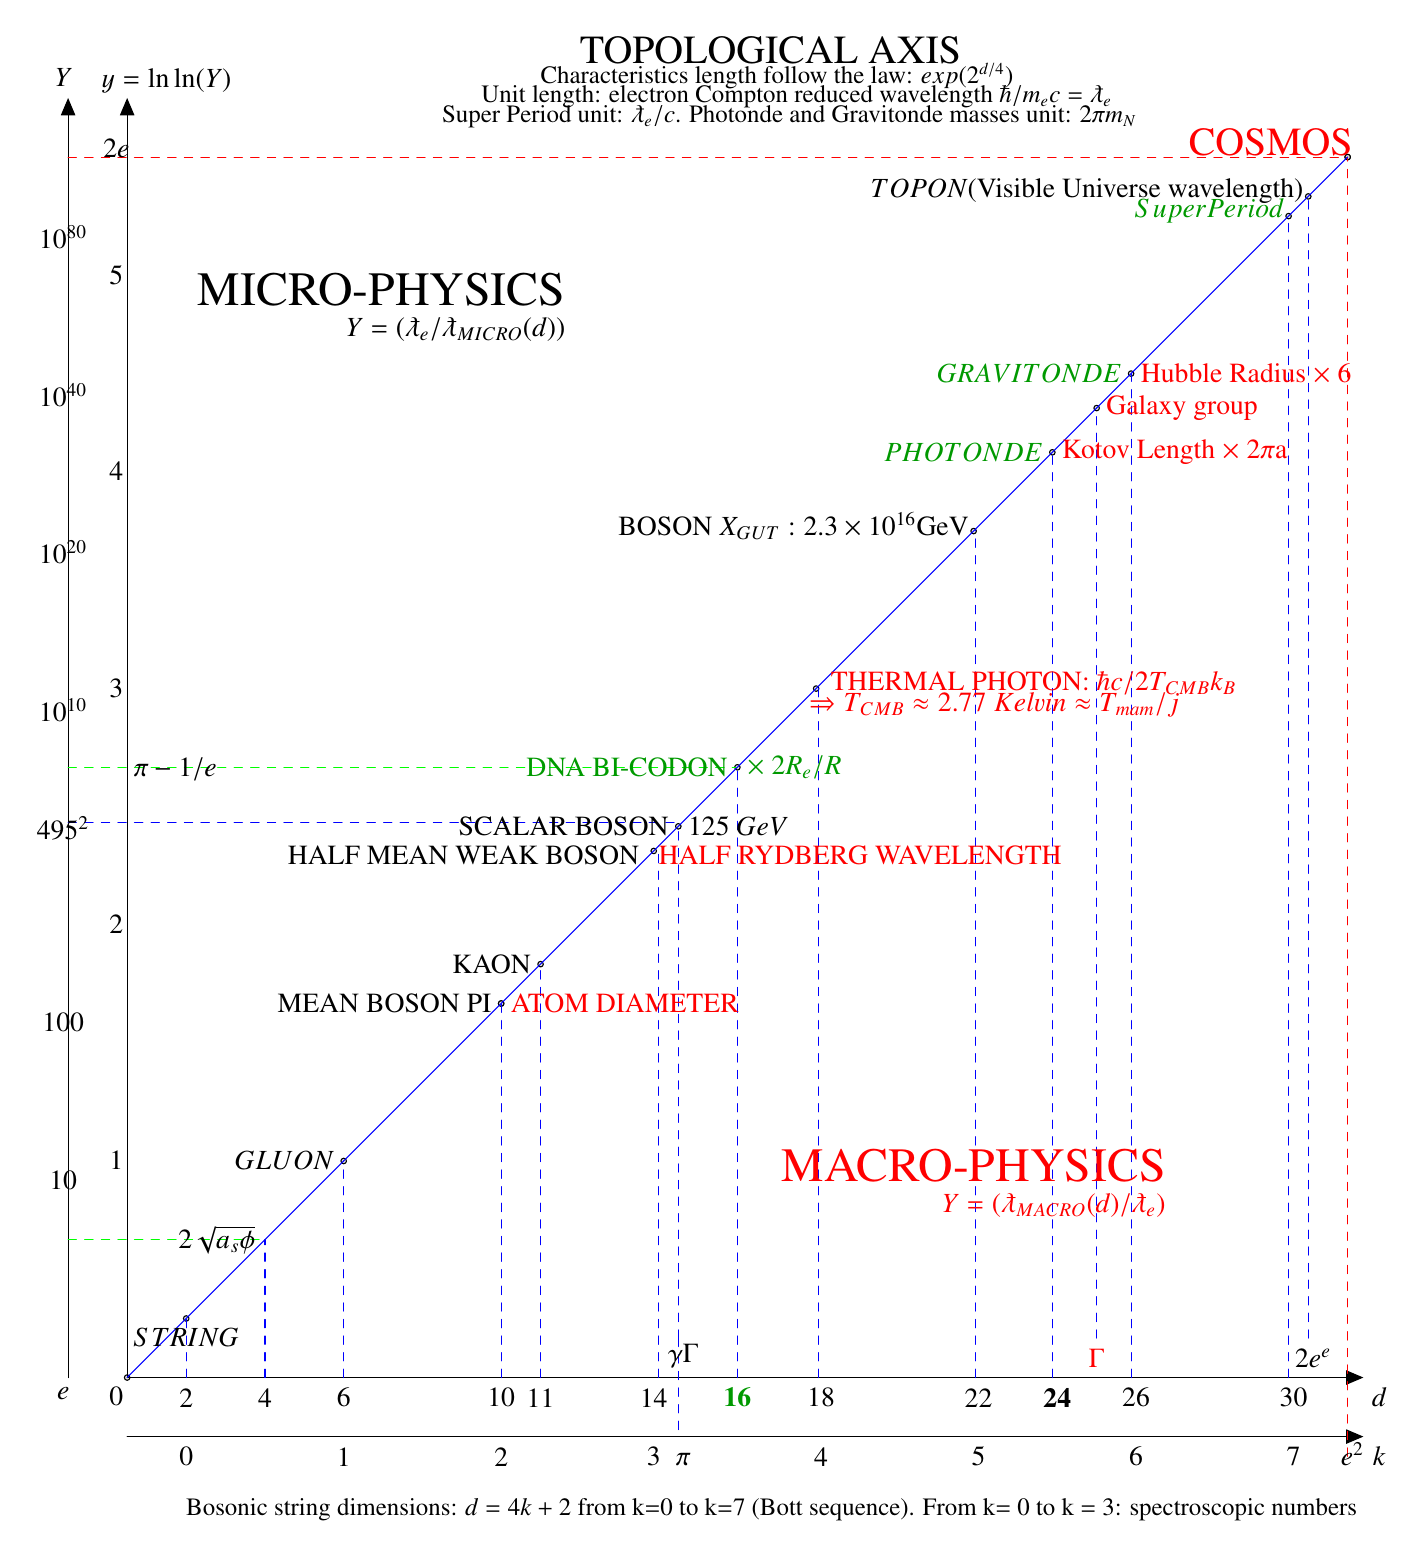
\begin{tikzpicture}[line cap=round,line join=round,>=triangle 
45,x=0.25cm,y=0.25cm]

\tkzDefPoint(-31.0,-31.0){A} %\tkzDefPoint(5.,3.43){B} \tkzDefPoint(5.,0.){C} \tkzDefPoint(31.0,31.0){Y}
\tkzDefPoint(-28.0,-28.0){B}
\tkzDefPoint(-20.0,-20.0){C}
\tkzDefPoint(-12.0,-12.0){D}
\tkzDefPoint(-12.0,-12.0){E}
\tkzDefPoint(28.0,28.0){F}
\tkzDefPoint(-4.25,-4.25){G}
\tkzDefPoint(4.0,4.0){H}
\tkzDefPoint(12.0,12.0){I}
\tkzDefPoint(-3.0,-3.0){J}
\tkzDefPoint(16.0,16.0){K}
\tkzDefPoint(18.25,18.25){L}
\tkzDefPoint(20.0,20.0){M}
\tkzDefPoint(29.0,29.0){N}
\tkzDefPoint(-10.0,-10.0){P}
\tkzDefPoint[color=red](31.0,31.0){Q}
\tkzDefPoint(31.0,31.0){Y}
\tkzDrawPoints(A,B,C,D,F,E,G,H,I,J,K,L,M,N,P,Q,Y)
%\tkzMarkRightAngle(A,D,C)
%\tkzLabelPoints[text=red,right](G,H)
%\tkzMarkAngle[fill=blue!40,size=1.4cm,opacity=.5](C,A,B)
%\tkzLabelAngle[pos=1.6](C,A,B){$\theta$}
\tkzDefMidPoint(A,Y) \tkzGetPoint{BI-CODON}
\coordinate (center) at (BI-CODON);
%\tkzLabelPoints[below,color=green](BICODON)
\tkzDrawPoints(BI-CODON)
\draw [->] (-31.0,-31.0) node[left]{} -- (-31.,34.) node[right]{}; % scale Y
%\draw [->] (31.0,-31.0) node[left]{} -- (31.,31.) node[right]{}; % 
\draw [->] (-31.0,-31.0) node[left]{} -- (31.8,-31.0) node[right]{}; % scale d
\draw [->] (-31.0,-34.) node[left]{} -- (31.8,-34.) node[right]{};   % scale k
\draw [->] (-34.0,-31.) node[left]{} -- (-34.,34.) node[right]{};   % scale Y'
%%% Blue Dashed Horizontal lines
\draw [-,color=green,dashed] (-34.0,-24.) node[left]{} -- (-24.,-24.) node[right]{};   % \sqrt{a_s} horizontal line
\draw [-,color=blue,dashed] (-34.0,-2.8) node[left]{} -- (-2.8,-2.8) node[right]{};   % Scalar Boson horizontal line
\draw [-,color=green,dashed] (-34.0,0.) node[left]{} -- (0.,0.) node[right]{};   % bicodon horizontal line
\draw [-,color=red,dashed] (-34.0,31.) node[left]{} -- (31.,31.) node[right]{};   % Cosmos horizontal line
%%% Blue Dashed Vertical lines
\draw [-,color=blue,dashed] (-28.0,-31.) node[left]{} -- (-28.,-28.) node[right]{};   % String vertical line
\draw [-,color=blue,dashed] (-24.0,-31.) node[left]{} -- (-24.,-24.) node[right]{};   % \sqrt{a_s} vertical line
\draw [-,color=blue,dashed] (-20.0,-31.) node[left]{} -- (-20.,-20.) node[right]{};   % Gluon vertical line
\draw [-,color=blue,dashed] (-12.0,-31.) node[left]{} -- (-12.,-12.) node[right]{};   % ATOM DIAMETER vertical line
\draw [-,color=blue,dashed] (-10.0,-31.) node[left]{} -- (-10.,-10.) node[right]{};   % Kaon vertical line
\draw [-,color=blue,dashed] (-4.0,-31.) node[left]{} -- (-4.,-4.) node[right]{};   % Half Mean Weak Boson vertical line
\draw [-,color=blue,dashed] (-3.0,-29.) node[left]{} -- (-3.,-3.) node[right]{};   % Scalar Boson vertical line
\draw [-,color=blue,dashed] (-3.0,-29.) node[left]{} -- (-3.,-34.) node[right]{};   % \gamma\Gamma->\pi vertical line
\draw [-,color=blue,dashed] (0.,-31.) node[left]{} -- (0.,0.) node[right]{};   % Bicodon vertical line
\draw [-,color=blue,dashed] (4.1,-31.) node[left]{} -- (4.1,4.1) node[right]{};   % Thermal Photon vertical line
\draw [-,color=blue,dashed] (12.1,-31.) node[left]{} -- (12.1,12.1) node[right]{};   % Boson X GUT vertical line
\draw [-,color=blue,dashed] (16.,-31.) node[left]{} -- (16.,16.) node[right]{};   % Photon vertical line
\draw [-,color=blue,dashed] (18.25,-29.) node[left]{} -- (18.25,18.25) node[right]{};   % Galaxy group vertical line
\draw [-,color=blue,dashed] (20.0,-31.) node[left]{} -- (20.0,20.) node[right]{};   % Gravitonde vertical line
\draw [-,color=blue,dashed] (28.0,-31.) node[left]{} -- (28.0,28.0) node[right]{};   % Super Period vertical line
\draw [-,color=blue,dashed] (29.,-29.) node[left]{} -- (29.,29.0) node[right]{};   % Topon vertical line
\draw [-,color=red,dashed] (31.0,-35.) node[left]{} -- (31.,31.) node[right]{};   % Cosmos vertical line

\draw[color=blue] (A) -- (Y);
\node [anchor = text=blue] at (-8.,35.75) {\Large{TOPOLOGICAL AXIS}};
\node [anchor = text=black] at (-10.,34.75) {\small{Characteristics length follow the law: $exp(2^{d/4})$}};
\node [anchor = text=black] at (-13.,33.75) {\small{Unit length: electron Compton reduced wavelength $\hbar /m_e c=\lambdabar_e$}};
\node [anchor = text=black] at (-15.,32.75) {\small{Super Period unit: $\lambdabar_e/c$. Photonde and Gravitonde masses unit: $2\pi m_N$}};
\node [anchor = text=black] at (-28.,-38.0) {\small{Bosonic string dimensions: $d=4k+2$ from k=0 to k=7 (Bott sequence). From k= 0 to k = 3: spectroscopic numbers}};
\node [anchor = east,text=red] at (31.75,31.75) {\Large{COSMOS}};
\node [anchor = south] at (-28.,-33.0) {$2$};
\node [anchor = south] at (-28.,-36.0) {$0$};
\node [anchor = north] at (-28.,-28.0) {$STRING$};

\node [anchor = south] at (-24.,-33.0) {$4$};
\node [anchor = east] at (-24.,-24.0) {$2\sqrt{a_s\phi}$};
\node [anchor = south] at (-20.,-33.0) {$6$};
\node [anchor = south] at (-20.,-36.0) {$1$};
\node [anchor = east] at (-20.,-20.0) {$GLUON$};
\node [anchor = south] at (-12.,-33.0) {$10$};
\node [anchor = south] at (-10.,-33.0) {$11$};
\node [anchor = south] at (-12.,-36.0) {$2$};
\node [anchor = east] at (-12.,-12.) {MEAN BOSON PI};
\node [anchor = west,color=red] at (-12.,-12.) {ATOM DIAMETER};
\node [anchor = east] at (-10.,-10.) {KAON};
\node [anchor = south] at (-4.25,-33.0) {$14$};
\node [anchor = south] at (-4.25,-36.0) {$3$};
\node [anchor = east] at (-4.5,-4.5) {HALF MEAN WEAK BOSON};
\node [anchor = west,color=red] at (-4.5,-4.5){HALF RYDBERG WAVELENGTH};
\node [anchor = south] at (-2.75,-31.0) {$\gamma\Gamma$};
\node [anchor = south] at (-2.75,-36.0) {$\pi$};
\node [anchor = east,color=black] at (-3.0,-3.0){SCALAR BOSON};
\node [anchor = west,color=black] at (-3.0,-3.0){$125~GeV$};
\node [anchor = south,color=black!40!green] at (0.,-33.0) {\textbf{16}};
\node [anchor = east,color=black!40!green] at (0.,0.0) {DNA BI-CODON};
\node [anchor = west,color=black!40!green] at (0.,0.0) {$\times~2R_e/R $};
%\node [anchor = west,color=black!40!green] at (0.,0.0) {$\times$ $2R_e/R\approx \mu^3\approx (\tau/\sqrt{e/2})^2$};
\node [anchor = south] at (4.25,-33.0) {$18$};
\node [anchor = south] at (4.25,-36.0) {$4$};
\node [cross,anchor = west,color=red] at (4.25,4.25){THERMAL PHOTON: $\hbar c/2T_{CMB}k_B$};
\node [cross,anchor = west,color=red] at (3.15,3.15){$\Rightarrow T_{CMB} \approx 2.77 ~Kelvin \approx T_{mam}/j$};
\node [anchor = south] at (12.25,-33.0) {$22$};
\node [anchor = south] at (12.25,-36.0) {$5$};
\node [anchor = east,color=black] at (12.25,12.250){BOSON $X_{GUT}:2.3 \times 10^{16}$GeV};
\node [anchor = east,color=black!40!green] at (16.,16.){$PHOTONDE$};
\node [anchor = west,color=red] at (16.,16.){Kotov Length $\times$ $2\pi$a};
\node [anchor = west,color=red] at (18.25,18.250){Galaxy group};
\node [anchor = south,color=red] at (18.25,-31.0) {$\Gamma$};
\node [anchor = east,color=black!40!green] at (20.,20.0){$GRAVITONDE$};
\node [anchor = west,color=red] at (20.,20.0){Hubble Radius $\times$ 6};
\node [anchor = south] at (16.25,-33.0) {\textbf{24}};
\node [anchor = east,color=black!40!green] at (28.25,28.250){$Super Period$};
\node [anchor = east,color=black] at (29.25,29.250){$TOPON$(Visible Universe wavelength)};
\node [anchor = east,color=black] at (-8.25,24.250){\LARGE{MICRO-PHYSICS}};
\node [anchor = east,color=black] at (-8.25,22.250){$Y=(\lambdabar_e/\lambdabar_{MICRO}(d))$};
\node [anchor = east,color=red] at (22.25,-20.250){\LARGE{MACRO-PHYSICS}};
\node [anchor = east,color=red] at (22.25,-22.250){$Y=(\lambdabar_{MACRO}(d)/\lambdabar_{e})$};
\node [anchor = south] at (20.25,-33.0) {$26$};
\node [anchor = south] at (20.25,-36.0) {$6$};
\node [anchor = south] at (28.25,-33.0) {$30$};
\node [anchor = south] at (28.25,-36.0) {$7$};
\node [anchor = south] at (31.25,-36.0) {$e^2$};
\node [anchor = south] at (29.25,-31.0) {$2e^e$};
\node [anchor = south] at (32.6,-33.00) {$d$};
\node [anchor = south] at (32.6,-36.00) {$k$};
%%% Y AXIS
\node [anchor = north] at (-31.55,-31.0) {$0$};
\node [anchor = north] at (-31.55,-19.0) {$1$};
\node [anchor = north] at (-31.55,-7.0) {$2$};
\node [anchor = north] at (-31.55, 5.0) {$3$};
\node [anchor = north] at (-28.55, 1.0) {$\pi-1/e$};
\node [anchor = north] at (-31.55, 16.0) {$4$};
\node [anchor = north] at (-31.55, 26.0) {$5$};
\node [anchor = north] at (-31.55, 32.4) {$2e$};
\node [anchor = north] at (-29.0,36.0) {$y=\ln\ln(Y)$};
%%% Y' AXIS
\node [anchor = north] at (-34.25,-31.0) {$e$};
\node [anchor = north] at (-34.25,-20.0) {$10$};
\node [anchor = north] at (-34.25,-12.0) {$100$};
\node [anchor = north] at (-34.25,-2.0) {$495^2$};
\node [anchor = north] at (-34.25,4.0) {$10^{10}$};
\node [anchor = north] at (-34.25,12.0) {$10^{20}$};
\node [anchor = north] at (-34.25,20.0) {$10^{40}$};
\node [anchor = north] at (-34.25,28.0) {$10^{80}$};
\node [anchor = north] at (-34.25,36.0) {$Y$};
%% SLOPE
%\tkzLabelSegment[sloped,below,text=black](A,D){Slope $\ln(2)/4$}
\end{tikzpicture}
{\color{black}
\caption[Graphics \ref{AxeTopologique}: Topological Axis ]{The main physical characteristics lengths $Y$, with unit length the electron reduced Compton wavelength: $\hbar/ m_ec=\lambdabar_e$, follows the law $exp(2^{d/4})$. This is the extrapolation of the Eddington's Large Number correlations, a reunion of height 2D-1D holographic relations, whose micro-macrophysics imbrication explains the double log, hence the name `Topological Axis'\cite{Sanchez2}. The double natural logarithms $y = ln(ln(Y))$ corresponds to the special string dimension series, which identifies with the spectroscopic series with spin 1/2, where $k$ is the orbital quantum number, $d = 4k + 2$, from $k = 0$ to $k = 7$, characteristics of a Bott octonion sequence. The mean value $d=16$ connects with the DNA bi-codon, decisive in the Holic Cosmology, where $R_e$ is the holographic reduced Cosmos radius and $R$ the Hubble radius. The mammal temperature $T_{mam}\approx j T_{CMB} $ connects directely with the Cosmos one $T_{CMB}$ where $j = 8\pi^2/ln2$ is the scale factor \cite{Sanchez3}. The ratio $R_e/R = pH/a^3$ is connected with the gauge couplings in Eq(9) while $e^4/4a_s$ is close to the Golden Number. $\Gamma=\gamma a/\pi$ is the Atiyah constant \cite{Atiyah}. The Kotov length is $ct_{nl}$. The Nambu mass, central in Particle Physics, is $m_N = a m_e$. In this rehabilitation of the Bosonic String Theory, the Universe appears as the final gauge boson in the Cosmos:  U (k = 7), GUT (k= 5), Weak (k=3), Gluon (k=1). }
}

\label{AxeTopologique}

\end{table}








\setcounter{page}{1}

\maketitle
%{\color{red} 
\begin{abstract}
 Dramatic confirmations of the previous article "Towards Science Unification through Number Theory" are presented. The Pell-Fermat and Lucas-Lehler numbers are central in confirming the liaison between the electrical constant $a$, the gauge couplings and the Topological Axis function. The cosmic Super-Period is confirmed by overwhelming correlations involving the Monster Group.

%The Number Theory comes back as the heart of unified Science, in a Computing Cosmos using the bases 2;3;5;7 whose two symmetric combinations explain the main lepton mass ratios. The corresponding Holic Principle induces a symmetry between the Newton and Planck constants which {\color{black} confirm} the Permanent Sweeping Holography Bang Cosmology, with invariant baryon density 3/10, the  baryons being dephased matter-antimatter oscillation. This implies the DNA bi-codon mean isotopic mass, confirming to 0.1 ppm the electron-based Topological Axis, whose terminal boson is the base 2 $c$-observable Universe in the base 3 Cosmos. The physical parameters involve the Euler idoneal numbers and the special Fermat primes of Wieferich (bases 2) and Mirimanoff (base 3). The prime numbers and crystallographic symmetries are related to the 4-fold structure of the DNA bi-codon. The forgotten Eddington's proton-tau symmetry is rehabilitated, renewing the supersymmetry quest. This excludes the concepts of Multiverse, Continuum, Infinity, Locality and Zero-mass Particle, leading to stringent predictions in Cosmology, Particle Physics and Biology. 
 
%}  
\end{abstract}

\keywords{ Number theory \and Optimal Computation Principle \and Holic Principle  \and Cosmology \and Supersymmetry  \and String Theory \and Bit-String Physics \and Cellular Automaton \and DNA nucleotides \and Crystallography \and Sporadic Groups.}

%In the recently published article (DOI 10.4236/apm.2021.111004), despite acute reading, several typos got wrong and some direct dramatict consequences were omitted. This Note resumes the main ones.




    



\begin{table}

\centering
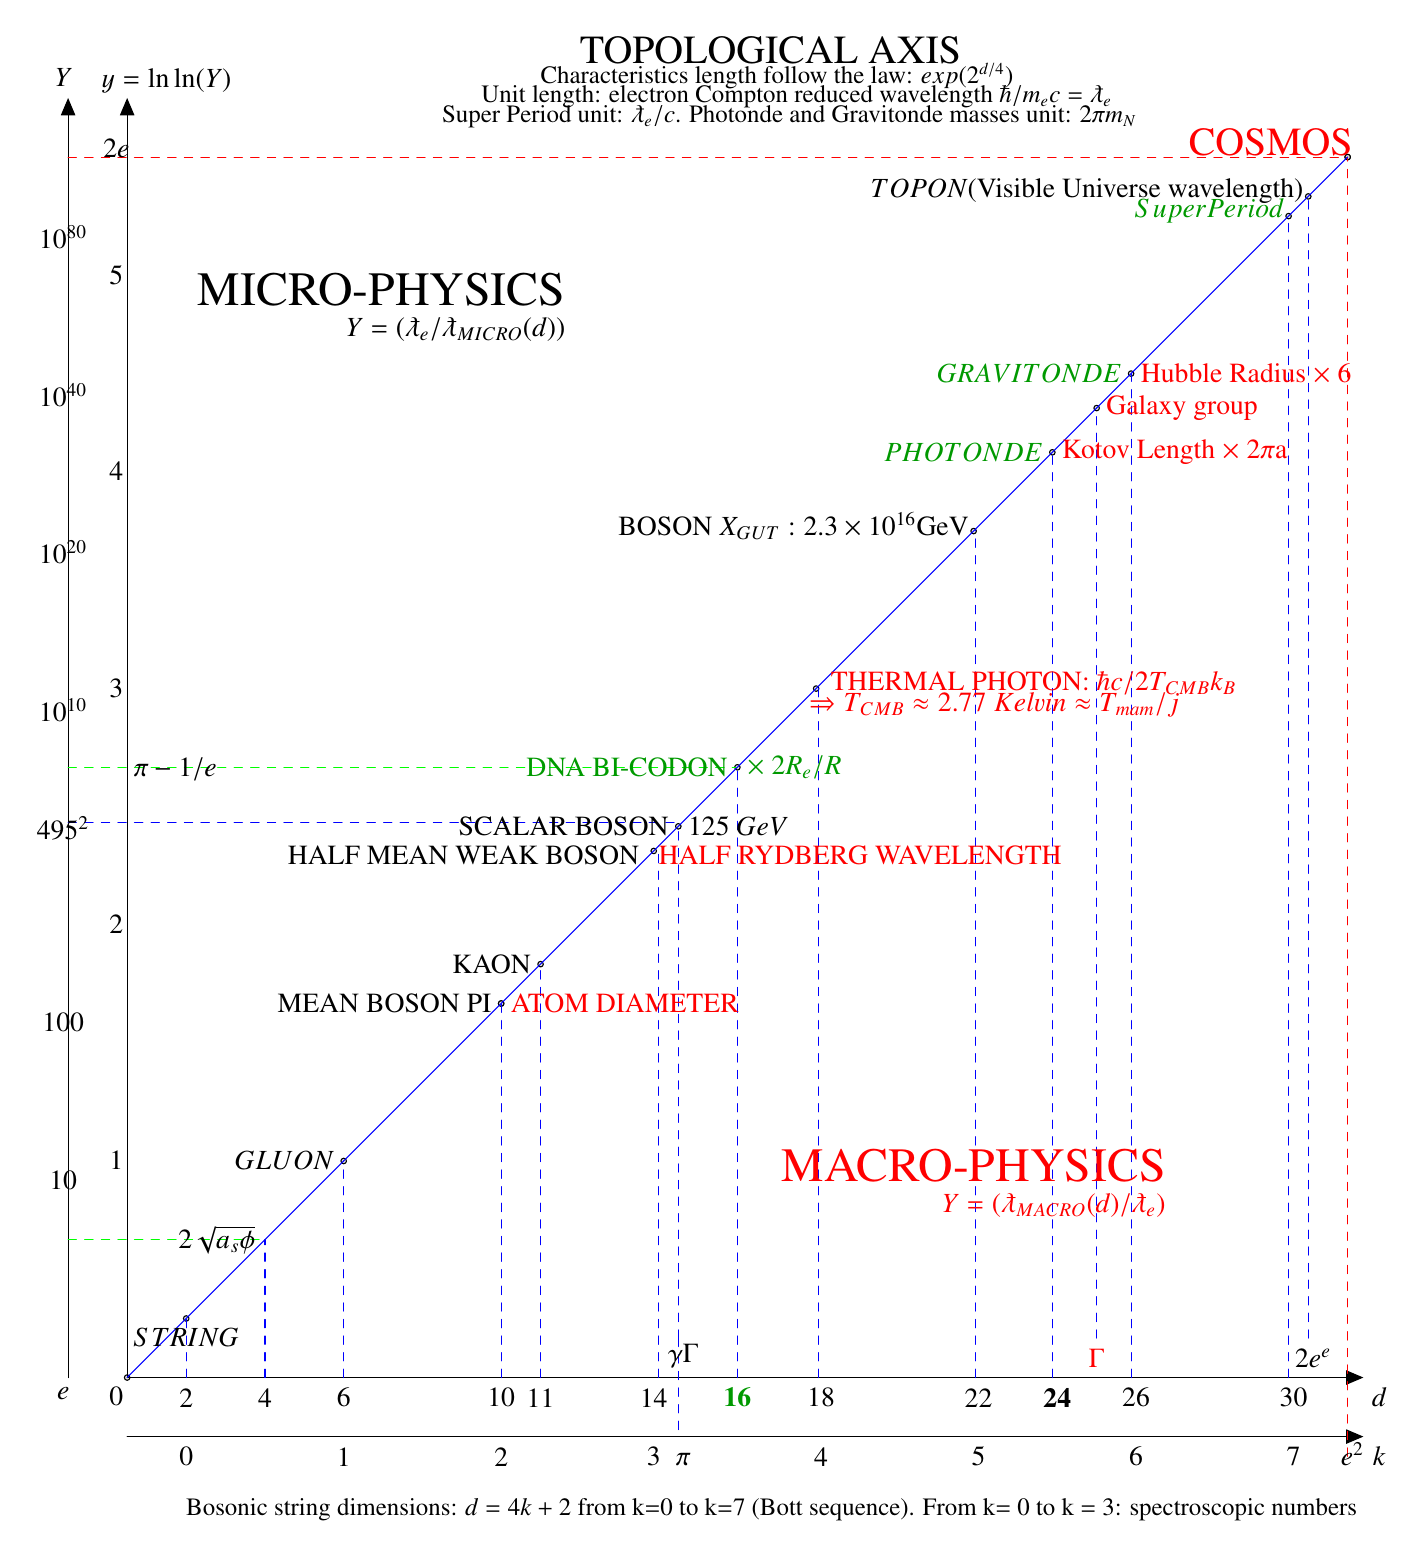
\begin{tikzpicture}[line cap=round,line join=round,>=triangle 
45,x=0.25cm,y=0.25cm]

\tkzDefPoint(-31.0,-31.0){A} %\tkzDefPoint(5.,3.43){B} \tkzDefPoint(5.,0.){C} \tkzDefPoint(31.0,31.0){Y}
\tkzDefPoint(-28.0,-28.0){B}
\tkzDefPoint(-20.0,-20.0){C}
\tkzDefPoint(-12.0,-12.0){D}
\tkzDefPoint(-12.0,-12.0){E}
\tkzDefPoint(28.0,28.0){F}
\tkzDefPoint(-4.25,-4.25){G}
\tkzDefPoint(4.0,4.0){H}
\tkzDefPoint(12.0,12.0){I}
\tkzDefPoint(-3.0,-3.0){J}
\tkzDefPoint(16.0,16.0){K}
\tkzDefPoint(18.25,18.25){L}
\tkzDefPoint(20.0,20.0){M}
\tkzDefPoint(29.0,29.0){N}
\tkzDefPoint(-10.0,-10.0){P}
\tkzDefPoint[color=red](31.0,31.0){Q}
\tkzDefPoint(31.0,31.0){Y}
\tkzDrawPoints(A,B,C,D,F,E,G,H,I,J,K,L,M,N,P,Q,Y)
%\tkzMarkRightAngle(A,D,C)
%\tkzLabelPoints[text=red,right](G,H)
%\tkzMarkAngle[fill=blue!40,size=1.4cm,opacity=.5](C,A,B)
%\tkzLabelAngle[pos=1.6](C,A,B){$\theta$}
\tkzDefMidPoint(A,Y) \tkzGetPoint{BI-CODON}
\coordinate (center) at (BI-CODON);
%\tkzLabelPoints[below,color=green](BICODON)
\tkzDrawPoints(BI-CODON)
\draw [->] (-31.0,-31.0) node[left]{} -- (-31.,34.) node[right]{}; % scale Y
%\draw [->] (31.0,-31.0) node[left]{} -- (31.,31.) node[right]{}; % 
\draw [->] (-31.0,-31.0) node[left]{} -- (31.8,-31.0) node[right]{}; % scale d
\draw [->] (-31.0,-34.) node[left]{} -- (31.8,-34.) node[right]{};   % scale k
\draw [->] (-34.0,-31.) node[left]{} -- (-34.,34.) node[right]{};   % scale Y'
%%% Blue Dashed Horizontal lines
\draw [-,color=green,dashed] (-34.0,-24.) node[left]{} -- (-24.,-24.) node[right]{};   % \sqrt{a_s} horizontal line
\draw [-,color=blue,dashed] (-34.0,-2.8) node[left]{} -- (-2.8,-2.8) node[right]{};   % Scalar Boson horizontal line
\draw [-,color=green,dashed] (-34.0,0.) node[left]{} -- (0.,0.) node[right]{};   % bicodon horizontal line
\draw [-,color=red,dashed] (-34.0,31.) node[left]{} -- (31.,31.) node[right]{};   % Cosmos horizontal line
%%% Blue Dashed Vertical lines
\draw [-,color=blue,dashed] (-28.0,-31.) node[left]{} -- (-28.,-28.) node[right]{};   % String vertical line
\draw [-,color=blue,dashed] (-24.0,-31.) node[left]{} -- (-24.,-24.) node[right]{};   % \sqrt{a_s} vertical line
\draw [-,color=blue,dashed] (-20.0,-31.) node[left]{} -- (-20.,-20.) node[right]{};   % Gluon vertical line
\draw [-,color=blue,dashed] (-12.0,-31.) node[left]{} -- (-12.,-12.) node[right]{};   % ATOM DIAMETER vertical line
\draw [-,color=blue,dashed] (-10.0,-31.) node[left]{} -- (-10.,-10.) node[right]{};   % Kaon vertical line
\draw [-,color=blue,dashed] (-4.0,-31.) node[left]{} -- (-4.,-4.) node[right]{};   % Half Mean Weak Boson vertical line
\draw [-,color=blue,dashed] (-3.0,-29.) node[left]{} -- (-3.,-3.) node[right]{};   % Scalar Boson vertical line
\draw [-,color=blue,dashed] (-3.0,-29.) node[left]{} -- (-3.,-34.) node[right]{};   % \gamma\Gamma->\pi vertical line
\draw [-,color=blue,dashed] (0.,-31.) node[left]{} -- (0.,0.) node[right]{};   % Bicodon vertical line
\draw [-,color=blue,dashed] (4.1,-31.) node[left]{} -- (4.1,4.1) node[right]{};   % Thermal Photon vertical line
\draw [-,color=blue,dashed] (12.1,-31.) node[left]{} -- (12.1,12.1) node[right]{};   % Boson X GUT vertical line
\draw [-,color=blue,dashed] (16.,-31.) node[left]{} -- (16.,16.) node[right]{};   % Photon vertical line
\draw [-,color=blue,dashed] (18.25,-29.) node[left]{} -- (18.25,18.25) node[right]{};   % Galaxy group vertical line
\draw [-,color=blue,dashed] (20.0,-31.) node[left]{} -- (20.0,20.) node[right]{};   % Gravitonde vertical line
\draw [-,color=blue,dashed] (28.0,-31.) node[left]{} -- (28.0,28.0) node[right]{};   % Super Period vertical line
\draw [-,color=blue,dashed] (29.,-29.) node[left]{} -- (29.,29.0) node[right]{};   % Topon vertical line
\draw [-,color=red,dashed] (31.0,-35.) node[left]{} -- (31.,31.) node[right]{};   % Cosmos vertical line

\draw[color=blue] (A) -- (Y);
\node [anchor = text=blue] at (-8.,35.75) {\Large{TOPOLOGICAL AXIS}};
\node [anchor = text=black] at (-10.,34.75) {\small{Characteristics length follow the law: $exp(2^{d/4})$}};
\node [anchor = text=black] at (-13.,33.75) {\small{Unit length: electron Compton reduced wavelength $\hbar /m_e c=\lambdabar_e$}};
\node [anchor = text=black] at (-15.,32.75) {\small{Super Period unit: $\lambdabar_e/c$. Photonde and Gravitonde masses unit: $2\pi m_N$}};
\node [anchor = text=black] at (-28.,-38.0) {\small{Bosonic string dimensions: $d=4k+2$ from k=0 to k=7 (Bott sequence). From k= 0 to k = 3: spectroscopic numbers}};
\node [anchor = east,text=red] at (31.75,31.75) {\Large{COSMOS}};
\node [anchor = south] at (-28.,-33.0) {$2$};
\node [anchor = south] at (-28.,-36.0) {$0$};
\node [anchor = north] at (-28.,-28.0) {$STRING$};

\node [anchor = south] at (-24.,-33.0) {$4$};
\node [anchor = east] at (-24.,-24.0) {$2\sqrt{a_s\phi}$};
\node [anchor = south] at (-20.,-33.0) {$6$};
\node [anchor = south] at (-20.,-36.0) {$1$};
\node [anchor = east] at (-20.,-20.0) {$GLUON$};
\node [anchor = south] at (-12.,-33.0) {$10$};
\node [anchor = south] at (-10.,-33.0) {$11$};
\node [anchor = south] at (-12.,-36.0) {$2$};
\node [anchor = east] at (-12.,-12.) {MEAN BOSON PI};
\node [anchor = west,color=red] at (-12.,-12.) {ATOM DIAMETER};
\node [anchor = east] at (-10.,-10.) {KAON};
\node [anchor = south] at (-4.25,-33.0) {$14$};
\node [anchor = south] at (-4.25,-36.0) {$3$};
\node [anchor = east] at (-4.5,-4.5) {HALF MEAN WEAK BOSON};
\node [anchor = west,color=red] at (-4.5,-4.5){HALF RYDBERG WAVELENGTH};
\node [anchor = south] at (-2.75,-31.0) {$\gamma\Gamma$};
\node [anchor = south] at (-2.75,-36.0) {$\pi$};
\node [anchor = east,color=black] at (-3.0,-3.0){SCALAR BOSON};
\node [anchor = west,color=black] at (-3.0,-3.0){$125~GeV$};
\node [anchor = south,color=black!40!green] at (0.,-33.0) {\textbf{16}};
\node [anchor = east,color=black!40!green] at (0.,0.0) {DNA BI-CODON};
\node [anchor = west,color=black!40!green] at (0.,0.0) {$\times~2R_e/R $};
%\node [anchor = west,color=black!40!green] at (0.,0.0) {$\times$ $2R_e/R\approx \mu^3\approx (\tau/\sqrt{e/2})^2$};
\node [anchor = south] at (4.25,-33.0) {$18$};
\node [anchor = south] at (4.25,-36.0) {$4$};
\node [cross,anchor = west,color=red] at (4.25,4.25){THERMAL PHOTON: $\hbar c/2T_{CMB}k_B$};
\node [cross,anchor = west,color=red] at (3.15,3.15){$\Rightarrow T_{CMB} \approx 2.77 ~Kelvin \approx T_{mam}/j$};
\node [anchor = south] at (12.25,-33.0) {$22$};
\node [anchor = south] at (12.25,-36.0) {$5$};
\node [anchor = east,color=black] at (12.25,12.250){BOSON $X_{GUT}:2.3 \times 10^{16}$GeV};
\node [anchor = east,color=black!40!green] at (16.,16.){$PHOTONDE$};
\node [anchor = west,color=red] at (16.,16.){Kotov Length $\times$ $2\pi$a};
\node [anchor = west,color=red] at (18.25,18.250){Galaxy group};
\node [anchor = south,color=red] at (18.25,-31.0) {$\Gamma$};
\node [anchor = east,color=black!40!green] at (20.,20.0){$GRAVITONDE$};
\node [anchor = west,color=red] at (20.,20.0){Hubble Radius $\times$ 6};
\node [anchor = south] at (16.25,-33.0) {\textbf{24}};
\node [anchor = east,color=black!40!green] at (28.25,28.250){$Super Period$};
\node [anchor = east,color=black] at (29.25,29.250){$TOPON$(Visible Universe wavelength)};
\node [anchor = east,color=black] at (-8.25,24.250){\LARGE{MICRO-PHYSICS}};
\node [anchor = east,color=black] at (-8.25,22.250){$Y=(\lambdabar_e/\lambdabar_{MICRO}(d))$};
\node [anchor = east,color=red] at (22.25,-20.250){\LARGE{MACRO-PHYSICS}};
\node [anchor = east,color=red] at (22.25,-22.250){$Y=(\lambdabar_{MACRO}(d)/\lambdabar_{e})$};
\node [anchor = south] at (20.25,-33.0) {$26$};
\node [anchor = south] at (20.25,-36.0) {$6$};
\node [anchor = south] at (28.25,-33.0) {$30$};
\node [anchor = south] at (28.25,-36.0) {$7$};
\node [anchor = south] at (31.25,-36.0) {$e^2$};
\node [anchor = south] at (29.25,-31.0) {$2e^e$};
\node [anchor = south] at (32.6,-33.00) {$d$};
\node [anchor = south] at (32.6,-36.00) {$k$};
%%% Y AXIS
\node [anchor = north] at (-31.55,-31.0) {$0$};
\node [anchor = north] at (-31.55,-19.0) {$1$};
\node [anchor = north] at (-31.55,-7.0) {$2$};
\node [anchor = north] at (-31.55, 5.0) {$3$};
\node [anchor = north] at (-28.55, 1.0) {$\pi-1/e$};
\node [anchor = north] at (-31.55, 16.0) {$4$};
\node [anchor = north] at (-31.55, 26.0) {$5$};
\node [anchor = north] at (-31.55, 32.4) {$2e$};
\node [anchor = north] at (-29.0,36.0) {$y=\ln\ln(Y)$};
%%% Y' AXIS
\node [anchor = north] at (-34.25,-31.0) {$e$};
\node [anchor = north] at (-34.25,-20.0) {$10$};
\node [anchor = north] at (-34.25,-12.0) {$100$};
\node [anchor = north] at (-34.25,-2.0) {$495^2$};
\node [anchor = north] at (-34.25,4.0) {$10^{10}$};
\node [anchor = north] at (-34.25,12.0) {$10^{20}$};
\node [anchor = north] at (-34.25,20.0) {$10^{40}$};
\node [anchor = north] at (-34.25,28.0) {$10^{80}$};
\node [anchor = north] at (-34.25,36.0) {$Y$};
%% SLOPE
%\tkzLabelSegment[sloped,below,text=black](A,D){Slope $\ln(2)/4$}
\end{tikzpicture}
{\color{black}
\caption[Graphics \ref{AxeTopologique}: Topological Axis ]{The main physical characteristics lengths $Y$, with unit length the electron reduced Compton wavelength: $\hbar/ m_ec=\lambdabar_e$, follows the law $exp(2^{d/4})$. This is the extrapolation of the Eddington's Large Number correlations, a reunion of height 2D-1D holographic relations, whose micro-macrophysics imbrication explains the double log, hence the name `Topological Axis'\cite{Sanchez2}. The double natural logarithms $y = ln(ln(Y))$ corresponds to the special string dimension series, which identifies with the spectroscopic series with spin 1/2, where $k$ is the orbital quantum number, $d = 4k + 2$, from $k = 0$ to $k = 7$, characteristics of a Bott octonion sequence. The mean value $d=16$ connects with the DNA bi-codon, decisive in the Holic Cosmology, where $R_e$ is the holographic reduced Cosmos radius and $R$ the Hubble radius. The mammal temperature $T_{mam}\approx j T_{CMB} $ connects directely with the Cosmos one $T_{CMB}$ where $j = 8\pi^2/ln2$ is the scale factor \cite{Sanchez3}. The ratio $R_e/R = pH/a^3$ is connected with the gauge couplings in Eq(9) while $e^4/4a_s$ is close to the Golden Number. $\Gamma=\gamma a/\pi$ is the Atiyah constant \cite{Atiyah}. The Kotov length is $ct_{nl}$. The Nambu mass, central in Particle Physics, is $m_N = a m_e$. In this rehabilitation of the Bosonic String Theory, the Universe appears as the final gauge boson in the Cosmos:  U (k = 7), GUT (k= 5), Weak (k=3), Gluon (k=1). }
}

\label{AxeTopologique}

\end{table}

\end{document}

